\chapter{Machine Learning} \label{chp:machinelearning}
\epigraph{In the early 1990's we were working with machine learning all the time, but back then we called it pattern recognition and regression.}{Prof. Anne Solberg, UiO}
\begin{figure}[H]
	\centering
	
\includegraphics[scale=0.4]{Images/example.png}
	\caption{Caption}
\end{figure}

\iffalse
Parameter estimation is a large part of science, because we are often not able to measure things directly. For instance, when Millikan in ... performed his famous electron charge experiment or when we estimate Sun's mass.
\fi 

The use of the term \textit{machine learning} has exploded over the past years, and sometimes it sounds like it is a totally new field. However, the truth is that many of the methods we use are relatively old, where for instance \textit{linear regression} was known early in the 19th century. \cite{legendre_nouvelles_1805}\cite{gauss_theoria_1809} Those methods have just recently been taken under the machine learning umbrella, which is one of the reasons why the term is mentioned so often. As the professor Anne Solberg at the University of Oslo pointed out during one of her lectures, problems where we want to minimize a cost function based on a set of parameters are today categorized as machine learning.

Another reason why machine learning has achieved .. the last few years, is that many of the algorithm have been dramatically improved. One of the most important contributions to this came in 2012, when the convolutional neural network (CNN) AlexNet won the \textbf{ImageNet Large Scale Visual Recognition Challenge} with the huge margin of 10.8\%. CITE ALEX Other important milestones are the improvement of reinforcement learning in order to solve problems, especially related to playing games and the recurrent neural networks (RNNs) for speech recognition, in particular the long short-term memory (LSTM) network. 

Unlike traditional algorithms, machine learning algorithms are not told what to do directly, but they use optimization tools to reproduce targets in the best way. As a consequence, we often do not know exactly what the algorithm does and why it behaves as is does, and because of this behavior, the processing is often called artificial intelligence. In our search for a technique to solve quantum mechanical problems where less physical intuition is needed, machine learning appears as a natural tool.

We usually distinguish between \textit{supervised} and \textit{unsupervised} learning, based on whether the model is trained on prior known targets or not. Even though the latter will be the most central part in our studies, the background theory of both techniques will be discussed carefully in this chapter. 

\section{Supervised Learning}
In supervised learning methods, we know the corresponding targets to the input data sets, which we use to train the model. This could for instance be linear regression, logistic regression or feed-forward neural networks.

Linear regression is perhaps the most intuitive example on this, where we want to find the line that fits some data points in the best possible way. In two dimensions, the $x$-coordinates are the inputs to the model and the $y$-coordinates are the targets. For instance, if we want to fit a second order polynomial,
\begin{equation}
f(x)=ax^2+bx+c,
\end{equation}
to a set of $n$ points $\{(x_1,y_1),(x_2,y_2),\hdots(x_n,y_n)\}$, one can set up a set of equations 
\begin{equation}
%\begin{vmatrix}
\mqty{
	\hat{y}_1&=&ax_1^2&+&bx_1&+&c\\
	\hat{y}_2&=&ax_2^2&+&bx_2&+&c\\
	\vdots&&\vdots&&\vdots&&\vdots\\
	\hat{y}_n&=&ax_n^2&+&bx_n&+&c
}
%\end{vmatrix}
\label{eq:lineareqs}
\end{equation}
where $\hat{y}_i$ is the $y$-value of the line at $x=x_i$. Our goal is to minimize the distance between $\hat{y}_i$ and $y_i$ by adjusting the parameters $a$, $b$ and $c$, which is usually done using the mean square error (MSE) as a measurement of the error. The cost function then reads
\begin{equation}
\mathcal{L}(a,b,c)=\sum_{i=1}^{n}\Big(y_i-(ax_i^2+bx_i+c)\Big)^2
\end{equation}
which can either be minimized by a matrix-vector product or an iterative minimization algorithm. Both these methods will be covered in the more general linear regression section below.

\subsection{Linear regression}
In linear regression, the dependent variable $y_i$ is a linear combination of the parameters, and for a dependent variable this can be written as
\begin{equation}
\hat{y}_i=\sum_jX_{ij}\beta_j
\label{eq:targets}
\end{equation}
where $\beta_j$'s are the unknown parameters to be found. In principle, $X_{ij}$ can be an arbitrary function of the arguments $x_i$, but in the polynomial case it can be simplified by setting $X_{ij} = x_i^j$. We will proceed dealing with $X_{ij}$ for general purposes.

The three most commonly used linear regression methods are \textit{ordinary least square} (OLS) regression, Ridge regression and Lasso regression, where the former has the cost function
\begin{empheq}[box={\mybluebox[5pt]}]{equation}
	\mathcal{L}(\bs{\beta})=\sum_{i=1}^{n}\Big(y_i-\beta_0-\sum_{j=1}^pX_{ij}\beta_j\Big)^2,\qquad\qquad\qquad\text{OLS}
\end{empheq}
which is minimized when
\begin{equation}
\bs{\beta}=(\hat{X}^T\hat{X})^{-1}\hat{X}^T\bs{y}.
\end{equation}

Quite often when we deal with large data sets, the design matrix contains singular values which give us problems with calculating $(\hat{X}^T\hat{X})^{-1}$. A way to avoid this is to introduce a penalty $\lambda$ to ensure that all the diagonal values are non-zero, which can be accomplished by adding a small value to all diagonal elements. This is the idea behind Ridge regression, which has the cost function
\begin{empheq}[box={\mybluebox[5pt]}]{equation}
	\mathcal{L}(\bs{\beta})=\sum_{i=1}^{n}\Big(y_i-\beta_0-\sum_{j=1}^pX_{ij}\beta_j\Big)^2+\lambda\sum_{j=1}^p\beta_j^2\qquad\text{Ridge}
\end{empheq}
and is minimized when
\begin{equation}
\bs{\beta}=(\hat{X}^T\hat{X}+\lambda I)^{-1}\hat{X}^T\bs{y}.
\end{equation}
Finally, we have Lasso regression with a cost function given by
\begin{empheq}[box={\mybluebox[5pt]}]{equation}
	\mathcal{L}(\bs{\beta})=\sum_{i=1}^{n}\Big(y_i-\beta_0-\sum_{j=1}^pX_{ij}\beta_j\Big)^2+\lambda\sum_{j=1}^p\beta_j\qquad\text{Lasso}
\end{empheq}
and without any expression for the optimized parameters. In order to optimize this cost function, we therefore need to use an iterative optimization algorithm. Such methods will later be used in the variational Monte-Carlo sampling, and some methods are therefore detailed in chapter \eqref{chp:optimization}. 

To illustrate how the iterative optimization works, we will go back to equation \eqref{eq:targets} and use OLS for simplicity reasons. Imagine that we have three points $\{(x_1,y_1),(x_2,y_2),(x_3,y_3)\}$ that we want to fit with a curve of two variables $\beta_1,\beta_2$. The simplest way to solve this interatively is to use \textbf{gradient descent} optimization, which goes as
\begin{equation}
\beta_k^+=\beta_k-\eta \frac{\partial\mathcal{L}(\bs{\beta})}{\partial\beta_k}
\end{equation}
with $\eta$ specifying how much the parameters should be changed for each iteration, known as the learning rate. 
The output $\hat{y}_i$ can be expressed by
\begin{equation}
\hat{y}_i=X_{i1}\beta_1+X_{i2}\beta_2
\end{equation}
and the network can be illustrated with $\beta_j$ as the input nodes, $\hat{y}_i$ as the output nodes and $X_{ij}$ as lines between all nodes, as in figure ... 

\subsection{Logistic regression}
Despite its name, logistic regression is not a fitting tool, but rather a classification tool. Traditionally, the perceptron model was used for 'hard classification', which sets the outputs directly to binary values. However, often we are interested in the probability of a given category, which means that we need a continuous \textit{activation function}. Logistic regression can, like linear regression, be considered as a function where coefficients are adjusted with the intention to minimize the error. Here, the coefficients are called \textit{weights}. The process goes like this: The inputs are multiplied by several weights, and by adjusting those weights the model can classify every \textit{linear classification problem}. A drawing of the perceptron is found in figure (\ref{fig:single_perceptron}).

\begin{tikzpicture}
\node[functions] (center) {};
\node[below of=center,text width=4em] {Activation function};
\draw[thick] (0.5em,0.5em) -- (0,0.5em) -- (0,-0.5em) -- (-0.5em,-0.5em);
\draw (0em,0.75em) -- (0em,-0.75em);
\draw (0.75em,0em) -- (-0.75em,0em);
\node[right of=center] (right) {};
\path[draw,->] (center) -- (right);
\node[functions,left=3em of center] (left) {$\sum$};
\path[draw,->] (left) -- (center);
\node[weights,left=3em of left] (2) {$w_2$} -- (2) node[input,left=2em of 2] (l2) {$X_{i2}$};
\path[draw,->] (l2) -- (2);
\path[draw,->] (2) -- (left);
\node[below of=2] (dots) {$\vdots$} -- (dots) node[left=2em of dots] (ldots) {$\vdots$};
\node[weights,below of=dots] (n) {$w_n$} -- (n) node[input,left=2em of n] (ln) {$X_{in}$};
\path[draw,->] (ln) -- (n);
\path[draw,->] (n) -- (left);
\node[weights,above of=2] (1) {$w_1$} -- (1) node[input,left=2em of 1] (l1) {$X_{i1}$};
\path[draw,->] (l1) -- (1);
\path[draw,->] (1) -- (left);
\node[weights,above of=1] (0) {$b$} -- (0) node[input,left=2em of 0] (l0) {$B$};
\node[right of=0] {bias};
\path[draw,->] (l0) -- (0);
\path[draw,->] (0) -- (left);
\node[below of=ln] {inputs};
\node[below of=n] {weights}; 
\end{tikzpicture}

In logistic regression, we usually have one binary output node for each class, but for two categories one output node is sufficient, which can be fired or not fired. 

Initially, one needs to train the perceptron such that it knows which outputs are correct, and for that one needs to know the outputs that correspond to the inputs. Every time the network is trained, the weights are adjusted such that the error is minimized.

The very first step is to calculate the initial outputs (forward phase), where the weights usually are set to small random numbers. Then the error is calculated, and the weights are updated to minimize the error (backward phase). So far so good.

\subsubsection{Forward phase}\label{sec:forward}
Let us look at it from a mathematical perspective, and calculate the net output. The net output seen from an output node is simply the sum of all the "arrows" that point towards the node, see figure (\ref{fig:single_perceptron}), where each "arrow" is given by the left-hand node multiplied with its respective weight. For example, the contribution from input node 2 to the output node follows from $X_2\cdot w_{2}$, and the total net output to the output $O$ is therefore
\begin{empheq}[box={\mybluebox[5pt]}]{equation}
	net = \sum_{i=1}^{I} x_i\cdot w_i + b\cdot 1.
	\label{eq:forward}
\end{empheq}
Just some notation remarks: $x_i$ is the value of input node $i$ and $w_{i}$ is the weight which connects input $i$ to the output. $b$ is the bias weight, which we will discuss later.

You might wonder why we talk about the net output all the time, do we have other outputs? If we look at the network mathematically, what we talk about as the net output should be our only output. Anyway, it turns out to be convenient mapping the net output to a final output using an activation function, which is explained further in section \ref{sec:sigmoid1}. The activation function, $f$, takes in the net output and gives the output, 
\begin{equation}
out = f(net).
\end{equation}
If not everything is clear right now, it is fine. We will discuss the most important concepts before we dive into the maths.

\subsubsection{BIAS}
As mentioned above, we use biases when calculating the outputs. The nodes, with value $B$, are called the bias nodes, and the weights, $b$, are called the bias weights. But why do we need those? 

Suppose we have two inputs of value zero, and one output which should not be zero (this could for instance be a NOR gate). Without the bias, we will not be able to get any other output than zero, and in fact the network would struggle to find the right weights even if the output had been zero. 

The bias value $B$ does not really matter since the network will adjust the bias weights with respect to it, and is usually set to 1 and ignored in the calculations. [2]

\subsubsection{Learning rate}
In principle, the weights could be updated without adding any learning rate ($\eta=1$), but this can in practice be problematic. It is easy to imagine that the outputs can be fluctuating around the targets without decreasing the error, which is not ideal, and a learning rate can be added to avoid this. The downside is that with a low learning rate the network needs more training to obtain the correct results (and it takes more time), so we need to find a balance. 

\subsubsection{Cost function}\label{sec:cost_function}
The cost function is what defines the error, and in logistic regression the cross-entropy function is a naturally choice. [3] It reads
\begin{empheq}[box={\mybluebox[5pt]}]{equation}
	c(\boldsymbol{W}) = -\sum_{i=1}^n\Big[y_i\log f(\boldsymbol{x}_i^T\boldsymbol{W})+(1-y_i)\log[1-f(\boldsymbol{x}_i^T\boldsymbol{W})]\Big]
	\label{eq:cross_entropy}
\end{empheq}
where $\bs{W}$ contains all weights, included the bias weight ($\bs{W}\equiv[b,\bs{W}]$), and similarly does $\bs{x}$ include the bias node, which is 1; $\bs{x}\equiv[1,\bs{x}]$. Further, the $f(x)$ is the activation function discussed in next section.

The cross-entropy function is derived from likelyhood function, which famously reads
\begin{equation}
p(y|x)=\hat{y}^y\cdot(1-\hat{y})^{1-y}.
\end{equation}
Working in the log space, we can define a log likelyhood function
\begin{align}
	\log\Big[p(y|x)\Big]&=\log\Big[\hat{y}^y\cdot(1-\hat{y})^{1-y}\Big]\\
	&=y\log\hat{y}+(1-y)\log(1-\hat{y})
\end{align}
which gives the log of the probability of obtaining $y$ given $x$. We want this quantity to increase then the cost function is decreased, so we define our cost function as the negative log likelyhood function. [7]

Additionally, including a regularization parameter $\lambda$ inspired by Ridge regression is often convenient, such that the cost function is
\begin{equation}
c(\bs{W})^+=c(\bs{W})+\lambda||\bs{W}||_2^2.
\end{equation}
We will later study how this regularization affects the classification accuracy. 

\subsubsection{Activation function}\label{sec:sigmoid1}
Above, we were talking about the activation function, which is used to activate the net output. In binary models, this is often just a step function firing when the net output is above a threshold. For continuous outputs, the logistic function given by
\begin{empheq}[box={\mybluebox[5pt]}]{equation}
	f(x)=\frac{1}{1+e^{-x}}.
	\label{eq:logistic}
\end{empheq}
is usually used in logistic regression to return a probability instead of a binary value. This function has a simple derivative, which is advantageous when calculating a large number of derivatives. As shown in section \ref{sec:sigmoid_der}, the derivative is simply
\begin{equation}
\frac{df(x)}{dx}=x(1-x).
\label{eq:logistic_der}
\end{equation}

$tanh(x)$ is another popular activation function in logistic regression, which more or less holds the same properties as the logistic function. 

\subsubsection{Backward phase}
Now all the tools for finding the outputs are in place, and we can calculate the error. If the outputs are larger than the targets (which are the exact results), the weights need to be reduced, and if the error is large the weights need to be adjusted a lot. The weight adjustment can be done by any minimization method, and we will look at a couple of gradient methods. To illustrate the point, we will stick to the \textbf{gradient descent} (GD) method in the calculations, even though other methods will be used later. The principle of GD is easy: each weight is "moved" in the direction of steepest slope,
\begin{empheq}[box={\mybluebox[5pt]}]{equation}
	\bs{w}^+= \bs{w} - \eta\cdot\frac{\partial c(\boldsymbol{w})}{\partial \bs{w}},
	\label{eq:w_update}
\end{empheq}
where $\eta$ is the learning rate and $c(\bs{w})$ is the cost function. We use the chain rule to simplify the derivative
\begin{equation}
\frac{\partial c(\bs{w})}{\partial \bs{w}} =\frac{\partial c(\bs{w})}{\partial out} \cdot\frac{\partial out}{\partial net} \cdot\frac{\partial net}{\partial \bs{w}}
\end{equation}
where the first is the derivative of the cost function with respect to the output. For the cross-entropy function, this is
\begin{equation}
\frac{\partial c(\bs{w})}{\partial out}=-\frac{y}{out}+\frac{1-y}{1-out}.
\end{equation}
Further, the second derivative is the derivative of the activation function with respect to the output, which is given in \eqref{eq:logistic_der}
\begin{equation}
\frac{\partial out}{\partial net}=out(1-out).
\end{equation}
The latter derivative is the derivative of the net output with respect to the weights, which is simply
\begin{equation}
\frac{\partial net}{\partial \bs{w}}=\bs{x}.
\end{equation}

If we now recall that $out=f(\bs{x}^T\bs{w})$, we can write 
\begin{equation}
\frac{\partial c(\bs{w})}{\partial \bs{w}}=[f(\bs{x}^T\bs{w})-\bs{y}]\bs{x}
\end{equation}
and obtain a weight update algorithm
\begin{empheq}[box={\mybluebox[5pt]}]{align}
	\bs{w}^+= \bs{w} - \eta\cdot[f(\bs{x}^T\bs{w})-\bs{y}]^T\bs{x}.
\end{empheq}
where the bias weight is included implicitly in $\bs{w}$ and the same applies for $\bs{x}$.

\subsection{Neural network} \label{sec:neural_network}
If you have understood logistic regression, understanding a neural network should not be a difficult task. According to  \textbf{the universal approximation theorem}, a neural network with only one hidden layer can approximate any continuous function. [8] However, often multiple layers are used since this tends to give fewer nodes in total. 

In figure \eqref{fig:neural_network}, a two-layer neural network (one hidden layer) is illustrated. It has some similarities with the logistic regression model in figure \eqref{fig:single_perceptron}, but a hidden layer and multiple outputs are added. In addition, the output is no longer probabilities and can take any number, which means that we do not need to use the logistic function on the outputs anymore.

\begin{tikzpicture}

% Define outputs
\node[] (center) {};
\node[input, above=0.3em of center] (y1) {$y_1$};
\node[input, below=0.3em of center] (y2) {$y_2$};

% Draw lines from output nodes
\node[right of=y1] (righty1) {};
\node[right of=y2] (righty2) {};
\path[draw,->] (y1) -- (righty1);
\path[draw,->] (y2) -- (righty2);

% Hidden nodes L
\node[input,left=5em of center] (aL3) {$a_3^{(L)}$};
\node[input,above of=aL3] (aL2) {$a_2^{(L)}$};
\node[input,above of=aL2] (aL1) {$a_1^{(L)}$};
\node[input,below of=aL3] (aL4) {$a_4^{(L)}$};
\node[input,below of=aL4] (aL5) {$a_5^{(L)}$};
\node[input,above of=aL1] (bL) {$B_L$};

% Hidden nodes 1
\node[input,left=25em of center] (a13) {$a_3^{(1)}$};
\node[input,above of=a13] (a12) {$a_2^{(1)}$};
\node[input,above of=a12] (a11) {$a_1^{(1)}$};
\node[input,below of=a13] (a14) {$a_4^{(1)}$};
\node[input,below of=a14] (a15) {$a_5^{(1)}$};
\node[input,above of=a11] (b1) {$B_1$};

% Hidden nodes l
\node[input,left=15em of center] (al3) {$a_3^{(l)}$};
\node[input,above of=al3] (al2) {$a_2^{(l)}$};
\node[input,above of=al2] (al1) {$a_1^{(l)}$};
\node[input,below of=al3] (al4) {$a_4^{(l)}$};
\node[input,below of=al4] (al5) {$a_5^{(l)}$};
\node[input,above of=al1] (bl) {$B_l$};

% Draw lines from hidden nodes
\path[draw,->] (aL1) -- (y1);
\path[draw,->] (aL2) -- (y1);
\path[draw,->] (aL3) -- (y1);
\path[draw,->] (aL4) -- (y1);
\path[draw,->] (aL5) -- (y1);
\path[draw,->] (bL) -- (y1);

\path[draw,->] (aL1) -- (y2);
\path[draw,->] (aL2) -- (y2);
\path[draw,->] (aL3) -- (y2);
\path[draw,->] (aL4) -- (y2);
\path[draw,->] (aL5) -- (y2) node[midway,below] {$w_{52}^{(L+1)}$};
\path[draw,->] (bL) -- (y2);

% Define place left of left
\node[input,left=5em of a13] (x2) {$x_2$};
\node[input,above of=x2] (x1) {$x_1$};
\node[input,below of=x2] (x3) {$x_3$};
\node[input,above of=x1] (b0) {$B_0$};

% Draw lines from input nodes
\path[draw,->] (x1) -- (a11);
\path[draw,->] (x1) -- (a12);
\path[draw,->] (x1) -- (a13);
\path[draw,->] (x1) -- (a14);
\path[draw,->] (x1) -- (a15);

\path[draw,->] (x2) -- (a11);
\path[draw,->] (x2) -- (a12);
\path[draw,->] (x2) -- (a13);
\path[draw,->] (x2) -- (a14);
\path[draw,->] (x2) -- (a15);

\path[draw,->] (x3) -- (a11);
\path[draw,->] (x3) -- (a12);
\path[draw,->] (x3) -- (a13);
\path[draw,->] (x3) -- (a14);
\path[draw,->] (x3) -- (a15) node[midway,below] {$w_{35}^{(1)}$};

\path[draw,->] (b0) -- (a11);
\path[draw,->] (b0) -- (a12);
\path[draw,->] (b0) -- (a13);
\path[draw,->] (b0) -- (a14);
\path[draw,->] (b0) -- (a15);

% Draw lines from first hidden layer
\path[draw,dashed,->] (a11) -- (al1);
\path[draw,dashed,->] (a11) -- (al2);
\path[draw,dashed,->] (a11) -- (al3);
\path[draw,dashed,->] (a11) -- (al4);
\path[draw,dashed,->] (a11) -- (al5);

\path[draw,dashed,->] (a12) -- (al1);
\path[draw,dashed,->] (a12) -- (al2);
\path[draw,dashed,->] (a12) -- (al3);
\path[draw,dashed,->] (a12) -- (al4);
\path[draw,dashed,->] (a12) -- (al5);

\path[draw,dashed,->] (a13) -- (al1);
\path[draw,dashed,->] (a13) -- (al2);
\path[draw,dashed,->] (a13) -- (al3);
\path[draw,dashed,->] (a13) -- (al4);
\path[draw,dashed,->] (a13) -- (al5);

\path[draw,dashed,->] (a14) -- (al1);
\path[draw,dashed,->] (a14) -- (al2);
\path[draw,dashed,->] (a14) -- (al3);
\path[draw,dashed,->] (a14) -- (al4);
\path[draw,dashed,->] (a14) -- (al5);

\path[draw,dashed,->] (a15) -- (al1);
\path[draw,dashed,->] (a15) -- (al2);
\path[draw,dashed,->] (a15) -- (al3);
\path[draw,dashed,->] (a15) -- (al4);
\path[draw,dashed,->] (a15) -- (al5) node[midway,below] {$w_{55}^{(l)}$};

\path[draw,dashed,->] (b1) -- (al1);
\path[draw,dashed,->] (b1) -- (al2);
\path[draw,dashed,->] (b1) -- (al3);
\path[draw,dashed,->] (b1) -- (al4);
\path[draw,dashed,->] (b1) -- (al5);

% Draw lines to last hidden layer
\path[draw,dashed,->] (al1) -- (aL1);
\path[draw,dashed,->] (al1) -- (aL2);
\path[draw,dashed,->] (al1) -- (aL3);
\path[draw,dashed,->] (al1) -- (aL4);
\path[draw,dashed,->] (al1) -- (aL5);

\path[draw,dashed,->] (al2) -- (aL1);
\path[draw,dashed,->] (al2) -- (aL2);
\path[draw,dashed,->] (al2) -- (aL3);
\path[draw,dashed,->] (al2) -- (aL4);
\path[draw,dashed,->] (al2) -- (aL5);

\path[draw,dashed,->] (al3) -- (aL1);
\path[draw,dashed,->] (al3) -- (aL2);
\path[draw,dashed,->] (al3) -- (aL3);
\path[draw,dashed,->] (al3) -- (aL4);
\path[draw,dashed,->] (al3) -- (aL5);

\path[draw,dashed,->] (al4) -- (aL1);
\path[draw,dashed,->] (al4) -- (aL2);
\path[draw,dashed,->] (al4) -- (aL3);
\path[draw,dashed,->] (al4) -- (aL4);
\path[draw,dashed,->] (al4) -- (aL5);

\path[draw,dashed,->] (al5) -- (aL1);
\path[draw,dashed,->] (al5) -- (aL2);
\path[draw,dashed,->] (al5) -- (aL3);
\path[draw,dashed,->] (al5) -- (aL4);
\path[draw,dashed,->] (al5) -- (aL5) node[midway,below] {$w_{55}^{(L)}$};

\path[draw,dashed,->] (bl) -- (aL1);
\path[draw,dashed,->] (bl) -- (aL2);
\path[draw,dashed,->] (bl) -- (aL3);
\path[draw,dashed,->] (bl) -- (aL4);
\path[draw,dashed,->] (bl) -- (aL5);

% Draw lines towards input nodes
\node[left of=x1] (leftx1) {};
\node[left of=x2] (leftx2) {};
\node[left of=x3] (leftx3) {};
\path[draw,->] (leftx1) -- (x1);
\path[draw,->] (leftx2) -- (x2);
\path[draw,->] (leftx3) -- (x3); 

% Add some text
\node[below=6.1em of x2] {input};
\node[below=6em of a13] {hidden 1};
\node[below=6em of al3] {hidden l};
\node[below=6em of aL3] {hidden L};
\node[below=6.8em of center] {output};
\end{tikzpicture}

Without a hidden layer, we have seen that the update of weights is quite straight forward. For a neural network consisting of multiple layers, the question is: how do we update the weights when we do not know the values of the hidden nodes? And how do we know which layer causing the error? This will be explained in section \ref{sec:backward}, where one of the most popular techniques for that is discussed. Before that we will generalize the forward phase presented in logistic regression.

\subsubsection{Forward phase}
In section \ref{sec:forward}, we saw how the output is found for a single perceptron. Since we only had one output node, the weights could be stored in an array. Generally, it is more practical to store the weights in matrices, since they will have indices related to both the node on left-hand side and the node on the right-hand side. For instance, the weight between input node $x_3$ and hidden node $h_5$ in figure \eqref{fig:neural_network} is usually labeled as $w_{35}$. Since we have two layers, we also need to denote which weight set it belongs to, which we will do by a superscript ($w_{35}\Rightarrow w_{35}^{(1)}$). In the same way, $\bs{W}^1$ is the matrix containing all $w_{ij}^{(1)}$, $\bs{x}$ is the vector containing all $x_i$'s and so on. We then find the net outputs at the hidden layer to be
\begin{empheq}{equation}
	net_{h,j} = \sum_{i=1}^{I} x_i\cdot w_{ij}^{(1)}=\bs{x}^T\bs{W}_j^{(1)}
	\label{eq:forward_hidden}
\end{empheq}
where the $\bs{x}$ and $\bs{W}^{(1)}$ again are understood to take the biases. This will be the case henceforth. The real output to the hidden nodes will be
\begin{equation}
h_j = f(net_{h,j}).
\end{equation}
Further, we need to find the net output to the output nodes, which is obviously just
\begin{empheq}{equation}
	net_{o,j} = \sum_{i=1}^{H} h_i\cdot w_{ij}^{(2)}=\bs{h}^T\bs{W}_j^{(2)}
	\label{eq:forward_output}
\end{empheq}
We can easily generalize this. Looking at the net output to a hidden layer $l$, we get
\begin{empheq}[box={\mybluebox[5pt]}]{equation}
	\bs{net}_{h_l} = \bs{h^{(l-1)}}^T\bs{W}^{(l)}.
	\label{eq:forward_general}
\end{empheq}

\subsubsection{Activation function}
Before 2012, the logistic, the tanh and the pur linear functions where the standard activation functions, but then Alex Krizhevsky published an article where he introduced a new activation function called \textit{Rectified Linear Units (ReLU)} which outperformed the classical activation functions. [4] The network he used is now known as AlexNet, and helped to revolutionize the field of computer vision. [5] After that, the ReLU activation function has been modified several times (avoiding zero derivative among others), and example of innovations are \textit{leaky ReLU} and \textit{Exponential Linear Unit (ELU)}. All those networks are linear for positive numbers, and small for negative numbers. Often, especially in the output layer, a straight linear function is used as well.

In figure (\ref{fig:activation_functions}), \textit{standard RELU, leaky RELU} and \textit{ELU} are plotted along with the logistic function.
\iffalse
\begin{figure} [H]
	\centering
	\subfloat[logistic]{{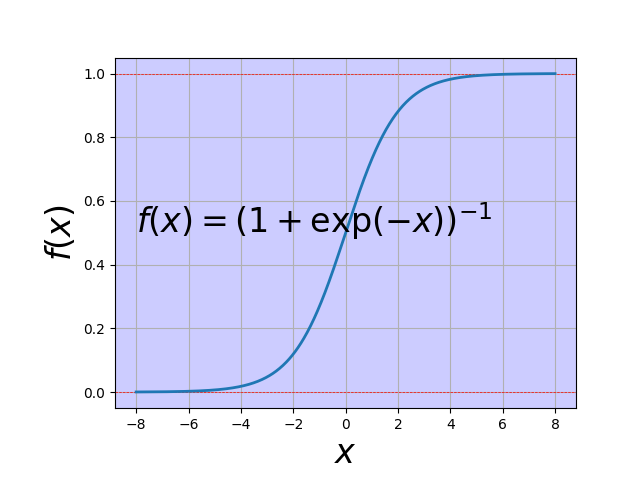
\includegraphics[width=8cm]{../plots/sigmoid.png} }}
	\subfloat[ReLU]{{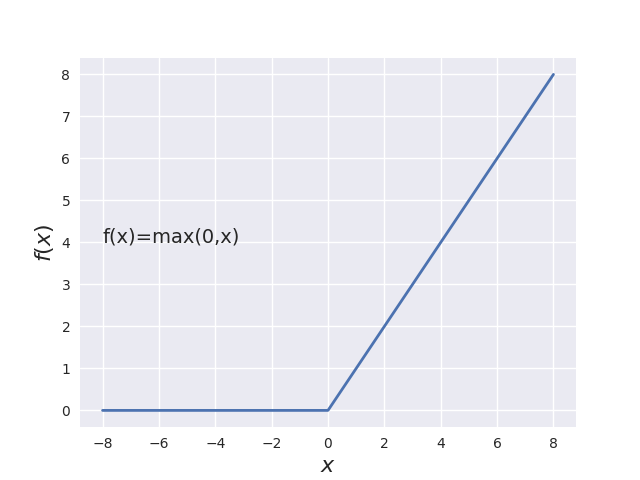
\includegraphics[width=8cm]{../plots/ReLU.png} }}\\
	
	\subfloat[Leaky ReLU]{{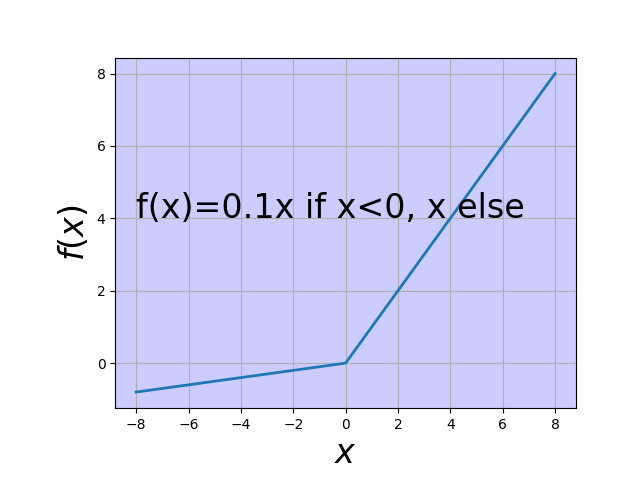
\includegraphics[width=8cm]{../plots/LeakyReLU.png} }}%
	\subfloat[ELU]{{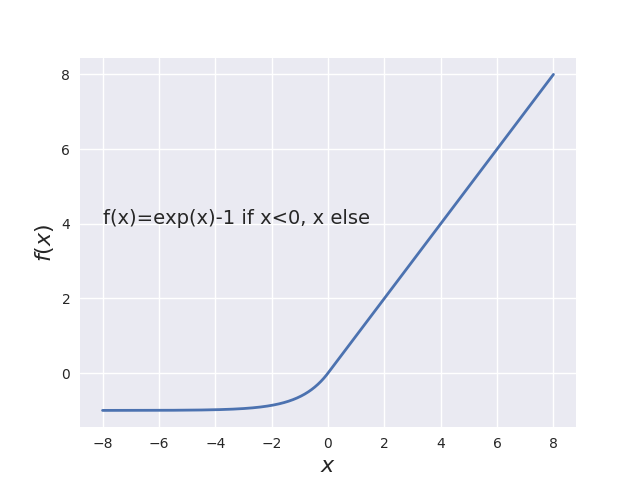
\includegraphics[width=8cm]{../plots/ELU.png} }}
	\caption{Some more or less popular activation functions}%
	\label{fig:activation_functions}%
\end{figure}
\fi

\subsubsection{Backward Propagation} \label{sec:backward}
Backward propagation is probably the most used technique for updating the weights, and is actually again based on equation (\ref{eq:w_update}). What differs, is the differentiation of the net input with respect to the weight, which gets more complex as we add more layers. For one hidden layer, we have two sets of weights, where the last layer is updated in a similar way as for a network without hidden layer, but the inputs are replaced with the values of the hidden nodes:
\begin{empheq}[box={\mybluebox[5pt]}]{align}
	w_{ij}^{(2)+}= w_{ij}^{(2)} - \eta\cdot[f(h_i^Tw_{ij})-y_j]^Th_i.
\end{empheq}
We recognize the first part as $\delta_{ok}$, such that
\begin{empheq}[box={\mybluebox[5pt]}]{equation}
	w_{ij}^{(1)+} = w_{ij}^{(1)} - \eta\cdot\sum_{k=1}^{O}\delta_{ok}\cdot w_{jk}^{(2)}\cdot f'(out_{hj})\cdot x_i
\end{empheq}
where we recall $\delta_{ok}$ as
\begin{equation*}
	\delta_{ok}=-(t_{ok}-out_{ok})\cdot f'(out_{ok}).
\end{equation*}
For more layers, the procedure is the same, but we keep on inserting the obtained outputs from various layers.

\subsubsection{Summary}
Since it will be quite a lot calculations, I will just express the results here, and move the calculations to Appendix B. The forward phase in a three-layer perceptron is
\begin{empheq}[box={\mybluebox[5pt]}]{align}
	net_{hi}&=\sum_jw_{ji}^{(1)}\cdot x_j\notag\\
	out_{hi}&=\text{f}(net_{hi})\notag\\
	\notag\\
	net_{ki}&=\sum_jw_{ji}^{(2)}\cdot out_{hj}\\
	out_{ki}&=\text{f}(net_{ki})\notag\\
	\notag\\
	net_{oi}&=\sum_jw_{ji}^{(3)}\cdot out_{kj}\notag\\
	out_{oi}&=\text{f}(net_{oi})\notag
\end{empheq}
which can easily be turned into vector form. The backward propagation follows from the two-layer example, and we get
\begin{empheq}[box={\mybluebox[5pt]}]{align}
	w_{ij}^{(3)}&=w_{ij}^{(3)}-\eta\cdot\delta_{oj}\cdot out_{ki}\notag\\
	\notag\\
	w_{ij}^{(2)}&=w_{ij}^{(2)}-\eta\sum_{k=1}^O\delta_{ok}\cdot w_{jk}^{(3)}\cdot f'(out_{kj})\cdot out_{hi}\notag\\
	\notag\\
	w_{ij}^{(1)}&=w_{ij}^{(1)}-\eta\sum_{k=1}^O\sum_{l=1}^K\delta_{ok}\cdot w_{lk}^{(3)}\cdot f'(out_{kl})\cdot w_{jl}^{(2)}f'(out_{hj})\cdot x_i\notag
\end{empheq}
where we again use the short hand 
\begin{equation*}
	\delta_{oj}=(t_j-out_{oj})\cdot f'(out_{oj}).
\end{equation*}
If we compare with the weight update formulas for the two-layer case, we recognize some obvious connections, and it is easy to imagine how we can construct a general weight update algorithm, no matter how many layers we have. 

Now over to the problem we want to solve using neural networks.


\section{Unsupervised Learning}
In unsupervised learning, a neural network is given the inputs only, and does not know what any target is. The task is then to find structures in the data, comparing data sets to each other and categorize the data sets with respect to their similarities and differences. 

Before we proceed to the unsupervised algorithms, we will dive into the statistics behind. After that, we will look at Boltzmann machines. 

\subsection{Statistical foundation}
FIRST explain why we need this probability... In unsupervised learning, it is all about probabilities.. We will stick to the continuous space, the discrete equivalent is just replacing the integrals with sums. 

The joint probability of measure both $x$ and $y$ is given by
\begin{equation}
p(x,y)=p(x|y)p(y)=p(y|x)p(x)
\label{eq:jointprob}
\end{equation}
where $p(x|y)$ and $p(y|x)$ are the conditional probabilities, and $p(x)$ and $p(y)$ are the marginal probabilities. By reordering equation \eqref{eq:jointprob}, we obtain Bayes' theorem
\begin{equation}
p(x|y)=\frac{p(y|x)p(x)}{p(y)}
\end{equation}
where $p(x)$ is the \textit{prior} probability, $p(y|x)$ is the \textit{likelyhood} and $p(x|y)$ is the \textit{posterior} probability. $p(y)$ can be sometimes found by an integral over the joint probability,
\begin{equation}
p(y)=\int dx p(x,y) = \int dx p(y|x)p(x),
\end{equation}
but often solving this integral is intractable. Different techniques require different approaches to this problem, and for our case we will use Markov chain Monte-Carlo methods to bypass it. More about that in section \eqref{chp:methods}. 

Next challenge is that we do not have the posterior

Kullback-Leibler divergence gives a measure of how much information is lost when one goes from one probability distribution to another. 

\subsection{Boltzmann Machines}
Boltzmann Machines are based on the more primitive Hopfield network, where a system of nodes is set up which defines the system energy. Inspired by statistical mechanics, the probability of finding the system in a state of energy $E$ is given by
\begin{equation}
p(\bs{x},\bs{h};\bs{\theta})=\frac{1}{Z(\bs{\theta})}\exp(-E(\bs{x},\bs{h};\bs{\theta})/k_BT)
\end{equation}
which is the Boltzmann distribution, hence the name Boltzmann machine. $k_B$ is known as Boltzmann's constant and $T$ is the system temperature, but henceforth they both will be omitted by scaling $E'(\bs{x},\bs{h};\bs{\theta})=E(\bs{x},\bs{h};\bs{\theta})/k_BT$. $Z(\bs{\theta})$ is known as the partition function, which is the sum over all possible probabilities.

\subsubsection{Marginal distributions}

\subsubsection{Conditional distributions}

In the most general form, all nodes are connected to all other nodes, that is an unrestricted Boltzmann machine, see figure \eqref{fig:boltzmann_machine} for illustration. 

\begin{tikzpicture}

% Define visible units
\node[input] (s2) {$s_2$};
\node[input] at (1,+3/2) (s1) {$s_1$};
\node[input] at (1,-3/2) (s3) {$s_3$};

% Define hidden units
\node[input] at (3,+3/2) (s6) {$s_6$};
\node[input] at (4,0) (s5) {$s_5$};
\node[input] at (3,-3/2) (s4) {$s_4$};

% Define biases
\node[input] at (2,7/2) (b) {$1$};

% Define paths
\path[draw,thick,-] (s1) -- (s2);
\path[draw,thick,-] (s2) -- (s3);
\path[draw,thick,-] (s3) -- (s4);
\path[draw,thick,-] (s4) -- (s5);
\path[draw,thick,-] (s5) -- (s6);
\path[draw,thick,-] (s6) -- (s1)  node[midway,above] {$w_{16}$};

\path[draw,thick,-] (s1) -- (s4);
\path[draw,thick,-] (s2) -- (s5);
\path[draw,thick,-] (s3) -- (s6);

\path[draw,thick,-] (s1) -- (s5);
\path[draw,thick,-] (s6) -- (s4);
\path[draw,thick,-] (s5) -- (s3);
\path[draw,thick,-] (s4) -- (s2);
\path[draw,thick,-] (s3) -- (s1);
\path[draw,thick,-] (s2) -- (s6);

\draw[color1,thick,-] (b) to [out=315,in=90] (s6); 
\draw[color1,thick,-] (b) to [out=225,in=90] (s1);
\draw[color1,thick,-] (b) to [out=337.5,in=90] (s5);
\draw[color1,thick,-] (b) to [out=202.5,in=90] (s2);
\draw[color1,thick,-] (b) to [out=0,in=0,distance=3cm] (s4);
\draw[color1,thick,-] (b) to [out=180,in=180,distance=3cm] (s3) node[] at (-1.5,0) {$b_3$};


% Add some text
%\node[below=1em of x3,font=\scriptsize] {visible};
%\node[below=1em of h3,font=\scriptsize] {hidden};
%\node[below=5.8em of center,font=\scriptsize] {output};
\end{tikzpicture}

In the same manner as for a feed-forward neural network, we can directly multiply each node $s_i$ with all its respective inner weights $w_{ij}$ and then with the other nodes $s_j$. To obtain the total system energy, we also need to include the bias weights, i.e, multiply $s_i$ with $b_i$. This gives the energy
\begin{equation}
E(\bs{s})=- \sum_{i=1}^Ns_ib_i-\sum_{i=1}^N\sum_{j=i}^N s_iw_{ij}s_j 
\label{eq:unrestrictedboltzmannmachine}
\end{equation}
for a system of $N$ nodes, which is the so-called binary-binary network and the most basic architecture. During training, the weights are adjusted in order to maximize the probability...

\subsection{Restricted Boltzmann machines}
When there is an unrestricted guy, a restricted guy must exist as well. What the term restricted means in this case, is that we ignore intra-layer connections and keep only the inter-layer ones. In the same manner as in equation \eqref{eq:unrestrictedboltzmannmachine}, we can look at the linear case, where each node is multiplied with the corresponding weight. We decide to split the bias nodes into one part connected to the \textit{visible} layer, $a_i$, and one part connected to the \textit{hidden} layer, $b_i$. The system energy then reads
\begin{equation}
E(\bs{x},\bs{h})=- \sum_{i=1}^Fx_ia_i- \sum_{j=1}^Hh_jb_j-\sum_{i=1}^F\sum_{j=i}^H x_iw_{ij}h_j 
\label{eq:binarybinary}
\end{equation}
which is the simplest type of units. $F$ is the number of visible nodes and $H$ is number of hidden nodes. The neural network is illustrated in figure \eqref{fig:restricted_boltzmann_machine}

\begin{tikzpicture}

% Define visible units
\node[input] (x2) {$x_2$};
\node[input] at (1,+3/2) (x1) {$x_1$};
\node[input] at (1,-3/2) (x3) {$x_3$};

% Define hidden units
\node[input] at (3,+3/2) (h1) {$h_1$};
\node[input] at (4,0) (h2) {$h_2$};
\node[input] at (3,-3/2) (h3) {$h_3$};

% Define biases
\node[input] at (0,7/2) (a) {$1$};
\node[input] at (4,7/2) (b) {$1$};

% Define paths
\path[draw,thick,-] (x1) -- (h1) node[midway,above] {$w_{11}$};
\path[draw,thick,-] (x1) -- (h2);
\path[draw,thick,-] (x1) -- (h3);

\path[draw,thick,-] (x2) -- (h1);
\path[draw,thick,-] (x2) -- (h2);
\path[draw,thick,-] (x2) -- (h3);

\path[draw,thick,-] (x3) -- (h1);
\path[draw,thick,-] (x3) -- (h2);
\path[draw,thick,-] (x3) -- (h3);

\draw[color3,thick,-] (b) to [out=270,in=90] (h1);
\draw[color3,thick,-] (b) to [out=315,in=45] (h2);
\draw[color3,thick,-] (b) to [out=0,in=0] (h3) node[] at (6,1) {$b_3$};

\draw[color1,thick,-] (a) to [out=270,in=90] (x1);
\draw[color1,thick,-] (a) to [out=225,in=135] (x2);
\draw[color1,thick,-] (a) to  [out=180,in=180] (x3) node[] at (-2,1) {$a_3$};


% Add some text
\node[below=1em of x3] {visible};
\node[below=1em of h3] {hidden};
\end{tikzpicture}


We can also take more complicated types of units into account than the binary-binary. A natural next step is the Gaussian-binary units, which has a Gaussian mapping between the visible node bias and the visible nodes. The simplest such structure gives the following system energy:

\begin{equation}
E(\bs{x},\bs{h})= \sum_{i=1}^F\frac{(x_i-a_i)^2}{2\sigma_i^2} - \sum_{j=1}^Hh_jb_j-\sum_{i=1}^F\sum_{j=i}^H \frac{x_iw_{ij}h_j}{\sigma_i^2} 
\label{eq:gaussianbinary}
\end{equation}
where $\sigma_i$ is the width of the Gaussian distribution, which can be set to an arbitrary number. 

\begin{equation}
\Psi(\bs{x};\bs{a},\bs{b},\bs{W})=\exp(-\sum_{i=1}^F\frac{(x_i-a_i)^2}{2\sigma^2})\prod_{j=1}^H\bigg(1+\exp\Big(b_j+\sum_{i=1}^F\frac{w_{ij}x_i}{\sigma^2}\Big)\bigg)
\label{eq:NQSWF}
\end{equation}
Need to compare it to standard VMC with Padé-Jastrow factor. 

\subsection{Partly restricted Boltzmann machine}
One can also imagine a partly restricted architecture, where we have inter-layer connections between the visible nodes, but not the hidden nodes. This is what we have decided to call a partly restricted Boltzmann machine. 

\begin{tikzpicture}

% Define visible units
\node[input] (x2) {$x_2$};
\node[input] at (1,+3/2) (x1) {$x_1$};
\node[input] at (1,-3/2) (x3) {$x_3$};

% Define hidden units
\node[input] at (3,+3/2) (h1) {$h_1$};
\node[input] at (4,0) (h2) {$h_2$};
\node[input] at (3,-3/2) (h3) {$h_3$};

% Define biases
\node[input] at (0,7/2) (a) {$1$};
\node[input] at (4,7/2) (b) {$1$}; 

% Define paths
\path[draw,thick,-] (x1) -- (h1) node[midway,above] {$w_{11}$};
\path[draw,thick,-] (x1) -- (h2);
\path[draw,thick,-] (x1) -- (h3);

\path[draw,thick,-] (x2) -- (h1);
\path[draw,thick,-] (x2) -- (h2);
\path[draw,thick,-] (x2) -- (h3);

\path[draw,thick,-] (x3) -- (h1);
\path[draw,thick,-] (x3) -- (h2);
\path[draw,thick,-] (x3) -- (h3);

\path[draw,color3,thick,-] (x1) -- (x2) node[midway, above left] {$c_{12}$};
\path[draw,color3,thick,-] (x2) -- (x3);
\path[draw,color3,thick,-] (x3) -- (x1); 

\draw[color2,thick,-] (b) to [out=270,in=90] (h1);
\draw[color2,thick,-] (b) to [out=315,in=45] (h2);
\draw[color2,thick,-] (b) to [out=0,in=0] (h3)  node[] at (6,1) {$b_3$};

\draw[color1,thick,-] (a) to [out=270,in=90] (x1);
\draw[color1,thick,-] (a) to [out=225,in=135] (x2);
\draw[color1,thick,-] (a) to [out=180,in=180] (x3) node[] at (-2,1) {$a_3$};

% Add some text
\node[below=1em of x3] {visible};
\node[below=1em of h3] {hidden};
\end{tikzpicture}


\begin{equation}
E(\bs{x},\bs{h})= \sum_{i=1}^F\frac{(x_i-a_i)^2}{2\sigma_i^2} - \sum_{i=1}^F\sum_{j=1}^Fx_ic_{ij}x_j- \sum_{j=1}^Hh_jb_j-\sum_{i=1}^F\sum_{j=i}^H \frac{x_iw_{ij}h_j}{\sigma_i^2} 
\label{eq:partlygaussianbinary}
\end{equation}

\begin{equation}
\Psi(\bs{x};\bs{a},\bs{b},\bs{W})=\exp(-\sum_{i=1}^F\frac{(x_i-a_i)^2}{2\sigma^2}+\sum_{i=1}^F\sum_{j=1}^Fx_ic_{ij}x_j)\prod_{j=1}^H\bigg(1+\exp\Big(b_j+\sum_{i=1}^F\frac{w_{ij}x_i}{\sigma^2}\Big)\bigg)
\label{eq:PNQSWF}
\end{equation}

\subsection{Deep Boltzmann machines}
...